\documentclass[12pt,a4paper]{article}

% Margins.
\setlength{\oddsidemargin}{0in}
\setlength{\evensidemargin}{0in}
\setlength{\headheight}{12pt}
\setlength{\headsep}{0pt}
\setlength{\topmargin}{-60pt}
\setlength{\textwidth}{6.5in}
\setlength{\textheight}{10.75in}

\usepackage{amsmath}
\usepackage{float}
\usepackage{graphicx}
\usepackage[hyphens]{url}
\usepackage{hyperref}	% Clickable links to figures, references and urls.
\usepackage{datetime}
\usepackage{longtable}

% Links direct to top of figures.
\usepackage[all]{hypcap}

% Drawing.
\usepackage{pgf}
\usepackage{tikz}

% Listings for formatting code.
\usepackage{listings}
\usepackage{textcomp}
% General options.
\lstset{breaklines=true, basicstyle=\small\ttfamily, tabsize=4, numbers=left, stepnumber=1, frame=single, showstringspaces=false, upquote=true}
% C++ specific high-lighting. Comments are 50/50 shades of green/black and strings coloured with 60/40 red/black mixture.
\lstset{language=[ISO]C++, commentstyle=\color{green!50!black}, keywordstyle=\color{blue}, stringstyle=\color{red!60!black}}

%opening
\title{Electromagnetic Theory\\Class 08\\Differential Length, Surface and Volume}
\author{Attique Dawood}
\date{September 10, 2014\\[0.2cm] Last Modified: \today, \currenttime}
\begin{document}
\maketitle
\section{Announcements}
\begin{itemize}
\item None.
\end{itemize}
\section{Revision}
\begin{itemize}
\item Vector conversions and transformation matrices.
\end{itemize}
\section{Differential Length, Surface and Volume Elements (3.2S)}
\subsection{Differential Length, Surface and Volume in Cartesian Coordinates}
In Cartesian coordinates a differential length element is generalised displacement in 3D space. Differential length is a vector. It is defined as,
\begin{equation}
d\textbf{\textit{l}}=dx\hat x+dy\hat y+dz\hat z
\end{equation}
The differential surface elements corresponding to $x=constant$, $y=constant$ and $z=constant$ planes are
\begin{equation}
\begin{split}
d\textbf{A}~\mathrm{or}~d\textbf{S}=~&dydz\hat x\\
&dxdz\hat y\\
&dxdy\hat z.
\end{split}
\end{equation}
The differential volume element is
\begin{equation}
dv=dxdydz
\end{equation}
\begin{figure}[H]
\centering
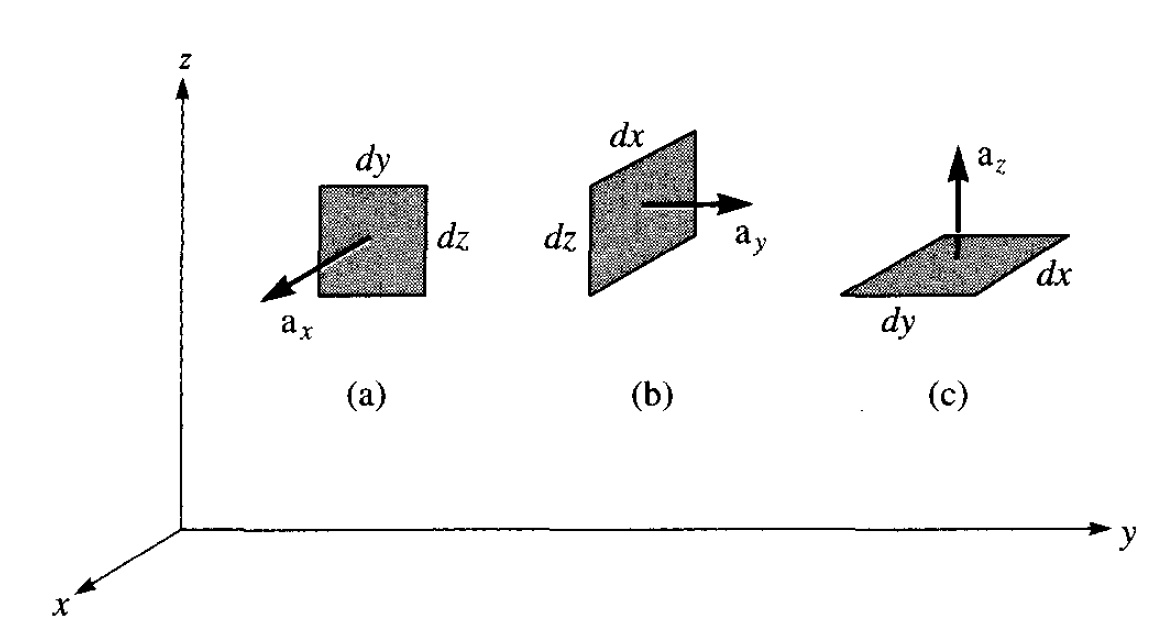
\includegraphics[scale=0.3]{Figure3-2S.png}
\caption{Differential normal areas in Cartesian coordinates. Figure taken from~\cite[Figure 3.2, page 54]{Sadiku}}
\label{Cartesian-differential-area}
\end{figure}
\subsection{Differential Length, Surface and Volume in Cylindrical Coordinates}
In Cylindrical coordinates differential length is defined as,
\begin{equation}
d\textbf{\textit{l}}=d\rho\hat \rho+\rho d\phi\hat \phi+dz\hat z
\end{equation}
Note that $d\phi$ is only an angle. Corresponding to a change in angle $d\phi$ the differential displacement/length is the arc length $\rho d\phi$. The differential surface elements corresponding to $\rho=constant$, $\phi=constant$ and $z=constant$ planes are
\begin{equation}
\begin{split}
d\textbf{A}~\mathrm{or}~d\textbf{S}=~&\rho d\phi dz\hat \rho\\
&d\rho dz\hat \phi\\
&\rho d\rho d\phi\hat z.
\end{split}
\end{equation}
The differential volume element is
\begin{equation}
dv=\rho d\rho d\phi dz
\end{equation}
\begin{figure}[htb]
\centering
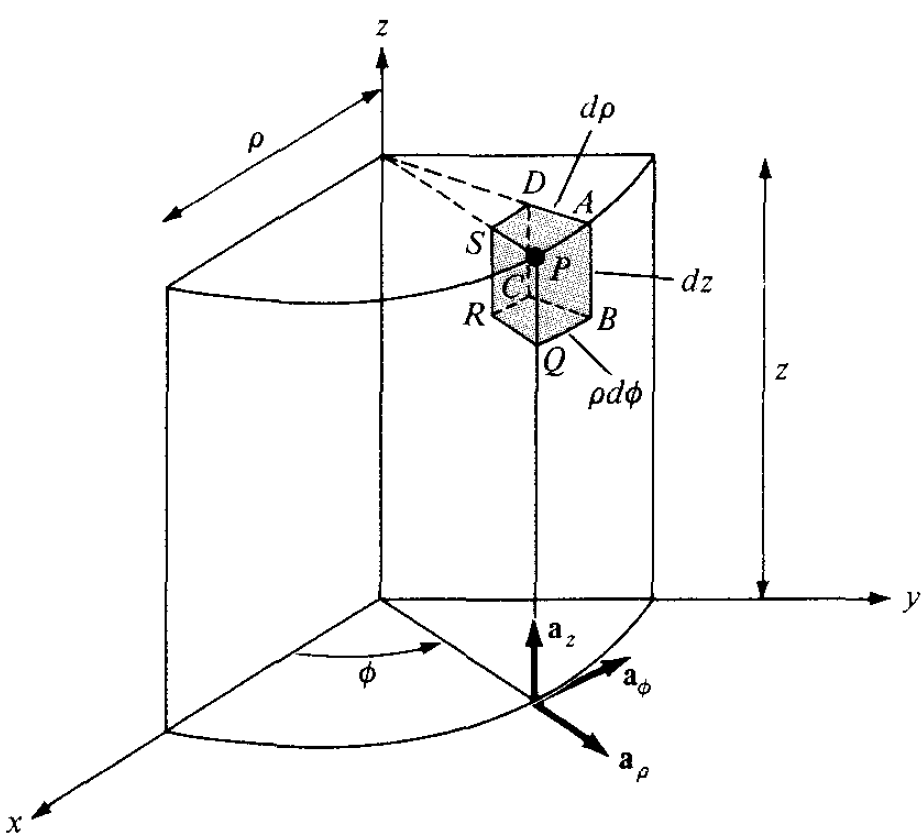
\includegraphics[scale=0.3]{Figure3-3S.png}
\caption{Differential volume in Cylindrical coordinates. Figure taken from~\cite[Figure 3.3, page 56]{Sadiku}}
\label{Cylindrical-differential-volume}
\end{figure}
\begin{figure}[htb]
\centering
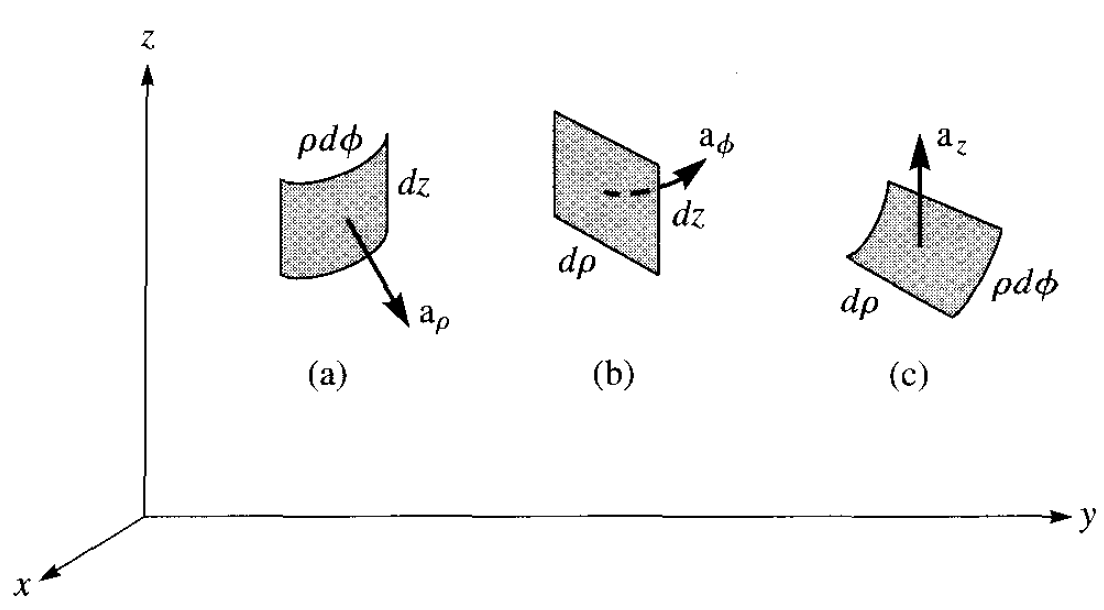
\includegraphics[scale=0.3]{Figure3-4S.png}
\caption{Differential normal areas in Cylindrical coordinates. Figure taken from~\cite[Figure 3.4, page 56]{Sadiku}}
\label{Cylindrical-differential-area}
\end{figure}
\subsection{Differential Length, Surface and Volume in Spherical Coordinates}
In Spherical coordinates differential length is defined as,
\begin{equation}
d\textbf{\textit{l}}=dr\hat r+r d\theta\hat \theta+r\sin\theta d\phi\hat \phi
\end{equation}
Note that $d\theta$ and $d\phi$ are angles. Corresponding to change in angles $d\theta$ and $d\phi$ the differential displacements are the arc lengths $rd\theta$ and $r\sin\theta d\phi$. Note that $\rho=r\sin\theta$ in Spherical coordinates. The differential surface elements corresponding to $r=constant$, $\theta=constant$ and $\phi=constant$ planes are
\begin{equation}
\begin{split}
d\textbf{A}~\mathrm{or}~d\textbf{S}=~&r^2\sin\theta d\theta d\phi\hat r\\
&r\sin\theta dr d\phi\hat\theta\\
&r dr d\theta\hat\phi.
\end{split}
\end{equation}
The differential volume element is
\begin{equation}
dv=r^2\sin\theta dr d\theta d\phi
\end{equation}
\begin{figure}[H]
\centering
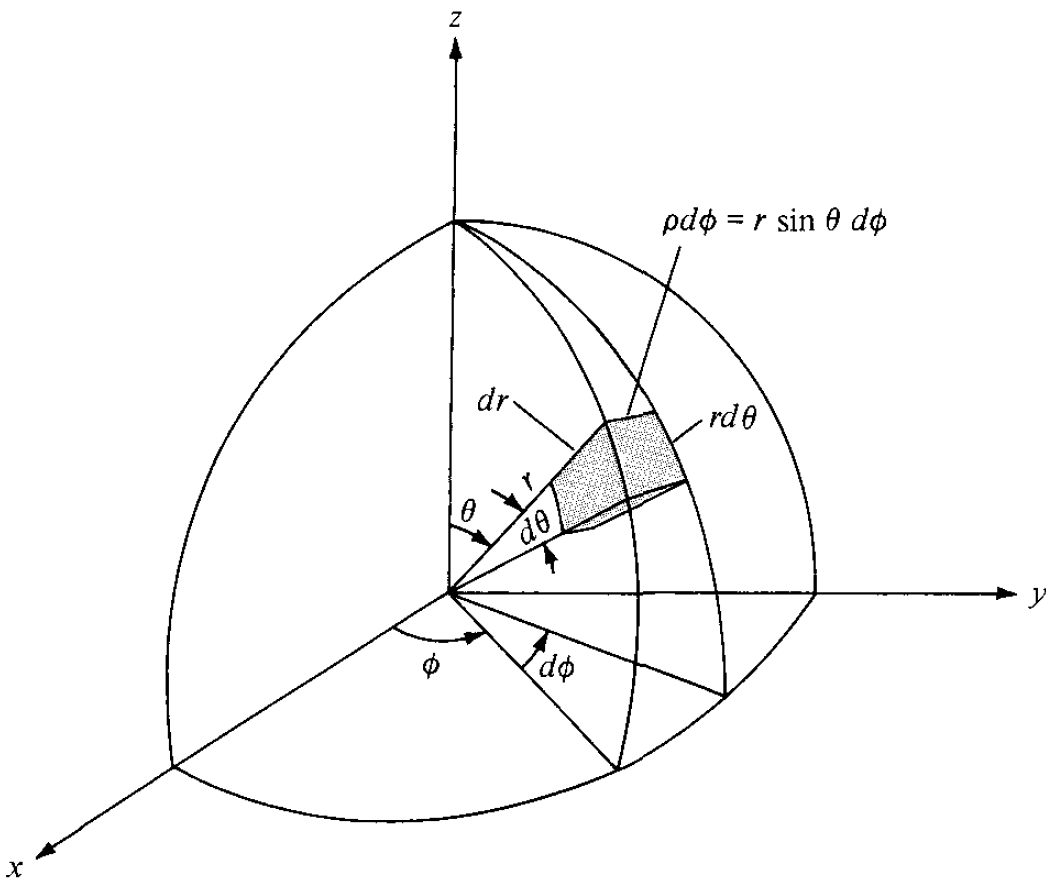
\includegraphics[scale=0.3]{Figure3-5S.png}
\caption{Differential volume in Spherical coordinates. Figure taken from~\cite[Figure 3.5, page 57]{Sadiku}}
\label{Spherical-differential-volume}
\end{figure}
\begin{figure}[h]
\centering
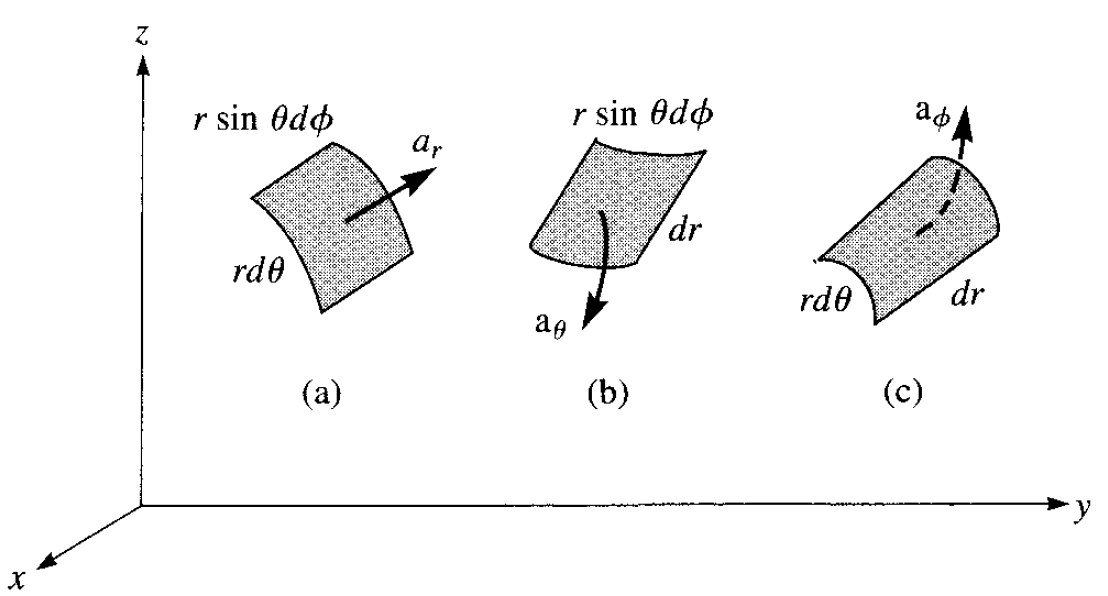
\includegraphics[scale=0.3]{Figure3-6S.png}
\caption{Differential normal areas in Spherical coordinates. Figure taken from~\cite[Figure 3.6, page 57]{Sadiku}}
\label{Spherical-differential-area}
\end{figure}
\section{Surface and Volume Integrals}
In electromagnetics we need to solve surface and volume integrals. Some common integrals are given below.
\begin{itemize}
\item $\int\limits_{S} d\mathrm{A}$~: Gives the total area of the surface `S'. This is generalised expression actually solved as a double integral.
\item $\int\limits_{v} dv$~: Calculate the total volume defined by limits of `v'. This is also a generalised expression actually solved as a triple integral.
\item $\int\limits_{S}\textbf{A}\cdot d\textbf{A}$~: Gives the total flux of the vector field \textbf{A} through the surface `S'.
\item $\int\limits_{v}\rho_v dv$~: If $\rho_v$ is volumetric charge density in $C/m^3$ then this integrals gives the total charge in volume `v'.
\end{itemize}
\section{Exercises}
\noindent\textbf{Question 1:} Use an appropriate $dS$ to find the surface area of given structures.
\begin{itemize}
\item[(1)] The area of curved surface of a cylinder of radius $\rho=3$ and height $0<z<2$.
\item[(2)] The surface area of a sphere of radius $r=3$.
\item[(3)] The area of curved surface of a slice of cake described by $\rho=3$, height $0<z<2$ and $0<\phi<30^0$.
\item[(4)] The area of an icecream cone described by $\theta=30^0$ and $0<r<3$.
\end{itemize}
\noindent\textbf{Question 2:} Use a suitable $dv$ to find the volumes of structures given in question 1.\\[0.2cm]
%\nocite{*}
\bibliographystyle{plain}
\bibliography{EMTRef}
\end{document}
